% !TeX root = ../main.tex

\chapter{POWERLINK通信协议研究}

实时以太网凭借其性能优势,不仅在工业领域得到广泛应用,在加速器控制领域的应用也越来越广泛。本章首先简介了实时以太网的发展情况,随后详细介绍了POWERLINK协议的通信机制、网络模型和数据帧结构,然后介绍了POWERLINK协议的基于PC和基于FPGA的两种实现方式,并搭建了相应的测试系统进行了性能测试,最后提出了理论分析和仿真建模两种方法对POWERLINK通信周期进行分析和评估。

\section{实时以太网介绍}

实时以太网是指在不改变ISO/IEC8802-3的通信特征、相关网络组件或 IEC1588 的总体行为基础上,通过一定程度的修改,使之满足实时行为。实时以太网既保持了普通以太网高通信速率等优势,又提高了其实时性、确定性、可靠性\cite{Hao2018}。根据实现机制和工业控制领域的实时性等级,实时以太网可以划分为class A、class B和class C三类\cite{wei2013},如图~\ref{fig:real-time Ethernet kinds}所示,一种实时以太网可以同时支持不同的技术实现方案,例如Ethernet/IP既有支持Class A的方案,也有支持Class C的方案。
Class A类别的实时以太网保持TCP/IP协议簇不变,保留传输层及以下的协议,只在应用层做了实时性修改,所以这种协议虽然可以直接接入普通以太网,但是并未克服普通以太网的原有缺陷,实时性不高,Modbus/TCP和Ethernet/IP实时以太网属于Class A类型的协议。Class B类别实时以太网弃用了TCP/IP的传输协议,在数据链路层及以上使用自定义的数据通信机制,物理层使用标准以太网的通信硬件,该类别实时以太网的实时性较强,一般可满足高性能的同步运动控制应用的实时需求,Ethernet POWERLINK、EPA和Profinet RT等实时以太网属于Class B类型的协议。Class C类别的实时以太网在数据链路层使用自定义的数据通信机制的同时,在物理层使用了专用的网络通信硬件,该类别实时性能最好,EtherCAT和Profinet IRT等实时以太网属于这类协议,Ethernet/IP为了提升性能,也有支持Class C类的技术方案。综合来看,在实时性能上,Class C优于CLass B,Class B优于Class A;在协议通用性上,Class A优于Class B,Class B优于CLass C。目前,在工业自动化领域有PROFINET、Ethernet POWERLINK、SERCOS III、EtherCAT 及EtherNet/IP 5个主流的实时以太网技术,以下分别做简单介绍。

\begin{figure}[!htb]
  \centering
  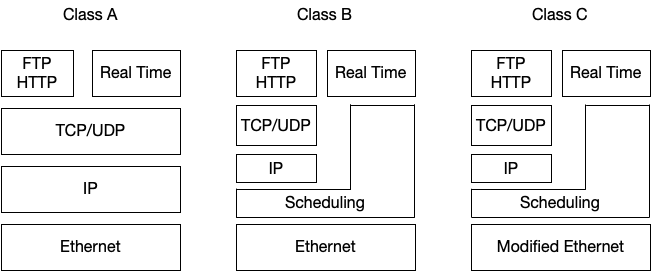
\includegraphics[width=\textwidth]{real-time-Ethernet-kinds.png}
  \caption{实时以太网分级}
  \label{fig:real-time Ethernet kinds}
\end{figure}

\subsubsection{Ethernet POWERLINK}
Ethernet POWERLINK(EPL)最初由奥地利B$\&$R公司于2001年11月创立和开发,自2003年以来,由独立的用户组织EPSG负责该技术的进一步发展\cite{ESPG},为了表述方便,本文将Ethernet POWERLINK简称为POWERLINK。EPSG在2008年发布了POWERLINK技术的开源版本openPOWERLINK,可在 PC、PLC、FPGA等硬件平台上实现\cite{oplk}。POWERLINK遵循IEEE1588分布式时钟系统标准,在数据链路层采用SCNM(Slot Communication Network Management)时间分片网络管理机制避免数据冲突从而进行高效的数据传输。具体来说,在POWERLNK通信网络中,只能指定一个设备为管理节点,其他设备为受控节点。管理节点为每个受控节点分配相应的通信时隙,每个管理节点只在自己的时隙内传输数据,互不干扰,这样可以保证在特定的时间内完成各节点的数据传输,满足实时性需求。

\subsubsection{PROFINET}
PROFINET是由 Profibus International 组织提出的实时以太网通信协议,PROFINET是基于IEEE 802.1D和IEEE 1588标准进行实时扩展\cite{Feld2005}。为满足不同工业场景下实时性需求,PROFINET提供了一个标准通信协议和SRT、IRT两种实时通信协议。标准通信协议是基于TCP/IP的协议,主要用于设备的参数化配置、组态和诊断数据的读取。SRT是软实时协议,SRT根据IEEE 802.1p标准定义了报文的优先级,主要用于数据的高性能循环传输。IRT协议的实现需要专用的等时同步ASIC芯片,适用于高性能数据传输和同步运动控制运用等场合。

\subsubsection{EtherCAT}
EtherCAT由德国Beckoff公司研发,由ETG组织维护发展。EtherCAT采用IEEE 1588标准实现分布式时钟精确同步,用于现场级的高速I/O网络,它的物理层使用标准的以太网物理层,可为双绞线和光纤\cite{Wang2011}。EtherCAT采用集总束帧等时通信的模式,主站负责把数据帧发送给各个从站,每个从站从该帧中取走属于自己的数据,或者写入该从站要输出的数据。从站在处理完成后会修改标志位,表明已完成数据帧的处理。

\subsubsection{SERCOS III}
SERCOS III是串行实时通信系统(Serial Real-time Communication System,SERCOS)的第三代协议,主要用于实现工控机与数字伺服系统、传感器和可编程控制器I/O口之间的实时数据通讯\cite{Wang2017}。与EtherCAT相同,SERCOS III采用集总束帧等时通信模式。虽然SERCOS III协议的通信循环周期最快可达到至31.25$\mu$s,但SERCOS III协议的物理层和数据链路层必须通过专用的SERCOS接口控制芯片实现。

\subsubsection{EtherNet/IP}
Ethernet/IP(Ethernet/Industrial Protocol)是由ControlNet组织CI、工业以太网协会IEA和供应商协会ODVA共同研发的,在标准的以太网硬件上运行,在TCP/IP和UDP/IP协议的基础上,在应用层采用CIP(Common Industrial Protocol)协议来进行实时数据交换\cite{Paul2001}。Ethernet/IP为了提升性能,也有支持Class C类的技术方案,2003年,ODVA通过制定CIPsync标准并推出专用以太网芯片,将EtherNet/IP的循环周期改善到百微秒量级,可用于伺服电机控制。

表~\ref{table:2.1}列出了上述5种主流工业以太网协议的性能。5种主流实时以太网技术在实时性方面的性能相当,循环周期都达到了100$\mu$s量级,可以满足加速器装置控制系统中对实时性的大部分需求。值得指出的是,在这5种主流实时以太网技术中,只有POWERLINK是完全开源的技术。POWERLINK 的开源性对粒子加速器控制系统来说具有特别重要的意义,开放和共享一直是粒子加速器控制技术的发展方向,所以本文采用POWERLINK实时以太网作为研究对象。

\begin{table}[!hbt]
  \centering\small
  \caption{5种主流工业以太网性能比较}
  \label{table:2.1} 
  \begin{tabular}{cccccc}
    \toprule

     &POWERLINK&PROFINET& EtherCAT &SERCOS III&EtherNet/IP\\
    \midrule
    发布时间& 2001& 2006 &2003& 2008& 2006\\
    
    冗余支持  &是& 是 &  否  &是  &是\\
    
    应用层协议 & CANopen&  Profibus&    CANopen&  SERCOS  &DeviceNet\\
    
    交叉通信  &是  &是  &   否 &否  &是\\
    
    循环周期  &100μs& 100μs&  100μs &100μs& 100μs\\
    
    抖动  &50-80ns & 20ns& 20ns  &50-80ns  &100ns\\
    
    技术实现& 无ASIC& ASIC&  ASIC  &ASIC&  无ASIC\\
    
    开放性 &主从开放 &从站开放&需购买授权 &主从开放 &主从开放\\
    
    通信模式  &轮询机制 &轮询机制&  集束帧&  集束帧 &轮询机制\\
    
    时钟标准& IEEE1588& IEEE1588& IEEE1588& IEEE1588& IEEE1588\\
    
    安全支持& openSAFETY &ProfiSafe &FEoE &SERCOS Safe& CIP Safety\\                  
    \bottomrule
  \end{tabular}

\end{table}

\section{POWERLINK协议介绍}

\subsection{POWERLINK协议的基本特性}

Ethernet POWERLINK协议遵循标准的OSI参考模型,与标准的以太网7层OSI参考模型不同的是POWERLINK仅定义了物理层、数据链路层和应用层三层协议,其中物理层和介质访问控制层与标准以太网相同,应用层采用工业控制领域常用的CANopen通信协议,为不同的应用提供兼容性接口。数据链路层采用SCNM机制来确保数据的实时性传输,SCNM机制即是时间片通信网络管理机制。SCNM的工作机制是将通信周期划分成不同的时间片段,并把这些时间段分配给等时同步数据和异步数据的传输,在等时同步数据传输阶段,网络中各节点只能在被分配的时间片段内传输数据,互不干扰。这种机制能够严格按照精确的时间片段来进行数据的传输,从而达到高实时性\cite{powerlink}。

Ethernet POWERLINK网络一般由一个主站和若干个从站组成,主站负责为从站分配时间片段和管理网络,又被称为管理节点(Management Node,MN),从站又被称为受控节点(Controlled Node,CN)。一个完整的EPL通信周期包括了等时同步通信阶段、异步通信阶段和空闲阶段。在等时同步通信阶段,主站会对各从站进行高精度的时钟同步,然后主站按照网络配置逐个轮询从站,从站接收到轮询请求后,才可以在属于自己的时间片段内传输数据。在异步通信阶段会进行一些非实时性数据或者其他协议的数据传输,包括基本的TCP/IP协议以及HTTP等应用层协议\cite{powerlink}。

基于POWERLINK协议的通信机制和网络结构,POWERLINK协议具有如下特性\cite{ESPG}:\\
(1) 开放性:POWERLINK协议代码开源,可在 PC、PLC、FPGA、ARM等硬件平台上实现;\\
(2) 实时性:在FPGA硬件平台下,最快通信循环周期<100$\mu$s;\\
(3) 抖动:网络抖动在50-80ns范围内;\\
(4) 兼容性:物理层基于IEEE 802.3标准以太网,支持标准以太网介质传输;应用层的CANopen协议支持大部分CANopen设备;\\
(5) 网络容量:一个EPL网络可以支持最多240个站点,每个站点可以支持最多1500个字节的吞吐量;\\
(6) 支持总线型、树型、星型、菊花链型等多种拓扑结构;\\
(7) 支持POWERLINK网络中各节点之间通信(交叉通信);\\
(8) 支持多主冗余、环网冗余和双网冗余等多种冗余方案;\\
(9) 引入openSAFETY技术,可应用于工业安全领域。

\subsection{POWERLINK协议的网络模型}
\label{subsection:POWERLINK协议的网络模型}

Ethernet POWERLINK协议的网络参考模型如图~\ref{fig:powerlink-arch}所示,主要有物理层、数据链路层和应用层组成。在添加了虚拟以太网接口之后,POWERLINK也可以支持TCP/IP协议簇,应用层也可以运行HTTP、FTP等协议。

\begin{figure}[!htb]
  \centering
  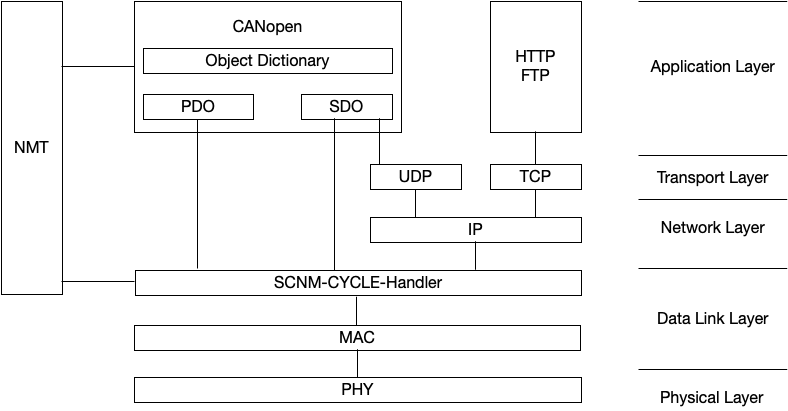
\includegraphics[width=\textwidth]{powerlink-arch.png}
  \caption{POWERLINK协议网络参考模型}
  \label{fig:powerlink-arch}
\end{figure}

\begin{itemize}
\item \textbf{物理层(PHY)} \\ 
POWERLINK协议的物理层和介质访问控制子层(MAC)是基于标准以太网的IEEE 802.3标准,工业领域较为常用的为百兆以太网,最新版本支持千兆以太网。POWERLINK网络支持总线型、树型、星型、菊花链型等多种拓扑结构,组网时为了保证数据的实时性,推荐使用集线器。集线器工作在物理层,抖动仅为几十纳秒,转发延时在亚微秒级别。网络连接器支持RJ45和M12两种类型,对于较恶劣的环境,可以使用M12接口和超6类线缆。

\item \textbf{数据链路层(Data Link Layer)} \\ 
POWERLINK网络中的通讯周期管理、时间片分配、时钟同步、数据报文的传输都是在数据链路层完成的。数据链路层定义了5种类型的协议帧,如表~\ref{table:2.2}所示,分别是SoC、PReq、PRes、SoA、Asnd。

\begin{table}[hbt]
  \centering
  \caption{Ethernet POWERLINK协议帧类型}
  \label{table:2.2}
  \setlength{\tabcolsep}{15mm}
  \begin{tabular}{cc}
    \toprule

     协议帧类型 & 协议帧名称\\
    \midrule
    周期开始 & SoC\\
    
    主站轮询请求 & PReq\\
    
    从站轮询响应 & PRes\\
    
    异步通信开始  & SoA\\
    
    从站异步响应  & Asnd\\              
    \bottomrule
  \end{tabular}

\end{table}

POWERLINK数据帧封装在标准以太网的数据段中,与标准以太网一致,POWERLINK数据帧长度最长为1518Byte,最短为64Byte。POWERLINK数据帧的结构如图~\ref{fig:message-arch}所示,其中0\textasciitilde13字节是标准以太网的帧头,n\textasciitilde n+4为CRC校验序列,14\textasciitilde n字节是POWERLINK数据帧信息。

\begin{figure}[!htb]
  \centering
  
\includegraphics[width=\textwidth]{message-arch.png}
  \caption{POWERLINK协议帧结构}
  \label{fig:message-arch}
\end{figure}

下面我们以SoC帧和PReq/PRes数据帧为例介绍POWERLINK数据帧的结构。SoC帧作为同步数据帧,帧长度固定为45Byte,其结构如图~\ref{fig:soa-message}所示,SoC数据帧中包含了网络绝对时间和相对时间,当主站为NMT\_GS\_INITIALISING状态时,相对时间清零,然后每产生一个 SOC,该数值就累加一个循环周期,其单位为$\mu$s。

\begin{figure}[!htb]
  \centering
  
\includegraphics[width=0.7\textwidth]{soa-message.png}
  \caption{SoA协议帧结构}
  \label{fig:soa-message}
\end{figure}

PReq作为主站发送给从站的请求数据帧,其结构如图~\ref{fig:preq-message}所示,其中包含了源站点站点号和用来寻址的目的站点号,从第10个字节开始是主站发送给从站的用户数据。PRes作为从站的响应数据帧通信数据帧,其结构和长度均与PReq数据帧类似,不同是是第5个字节中包含了异步发送队列中数据帧的优先级和队列中挂起的数据帧数目。

\begin{figure}[!htb]
  \centering
  
\includegraphics[width=0.7\textwidth]{preq-message.png}
  \caption{PReq协议帧结构}
  \label{fig:preq-message}
\end{figure}

一个基本的POWERLINK通信周期分为三个阶段,按发生顺序分别是等时同步阶段、异步通信阶段和空闲阶段,通信过程如图~\ref{fig:communication-process}所示。等时同步阶段用来传输周期性的实时数据,主站首先通过以太网广播发送SoC帧对所有从站进行时钟同步,然后通过PReq帧依次轮询每个已配置的处于活动状态的从站。PReq帧仅被节点号对应的从站接收,对应的的从站通过PRes广播帧响应此请求。若有从站在一定时间内未做出响应,则主站不会因此中断通信,会继续轮询之后的从站。在异步通信阶段,仅一个被授权的从站可以在此阶段传输非实时数据。主站首先广播SoA帧,被授权的从站向网络中发送Asnd帧回应。异步通信阶段不是必须的,没有异步通信阶段的情况下,等时同步阶段之后会直接进入空闲阶段。空闲阶段是本周期数据传输完成后与下一个周期开始之间的时间间隔。


\begin{figure}[!htb]
  \centering
  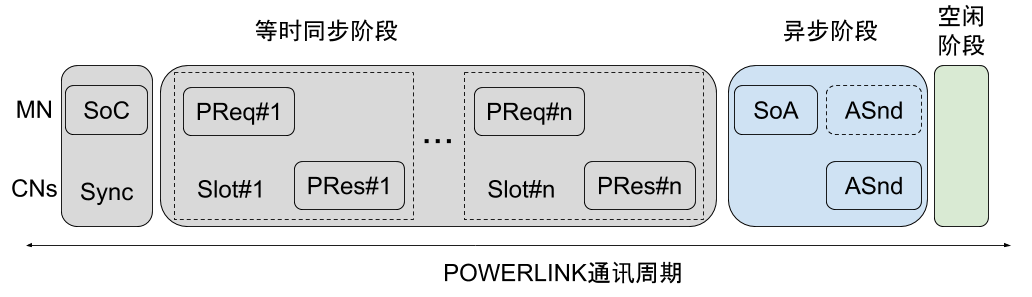
\includegraphics[width=\textwidth]{communication-process.png}
  \caption{POWERLINK通讯过程}
  \label{fig:communication-process}
\end{figure}

\item \textbf{应用层(Application Layer)} \\ 
POWERLINK的应用层时遵循CANOpen标准,其核心是对象字典(OBD)\cite{jin2012}。OBD是一种数据结构,其中包含与通信协议相关的所有参数以及通信中的过程变量。在POWERLINK网络中,周期性实时传输的OBD对象被映射为过程数据对象(PDO),PDO分为两类:发送过程数据对象(TPDO)和接收过程数据对象(RPDO),分别是该站的发送数据和接收数据的载体。非实时性的OBD对象(例如网络配置命令)被映射为服务数据对象(SDO)。

\end{itemize}

\section{POWERLINK协议的实现}

Ethernet POWERLINK协议作为一种开源的实时以太网技术可以在多种平台下实现,本章重点研究了POWERLINK协议实现方案之一的openPOWERLINK。openPOWERLINK是由德国SYSTEC电子、B$\&$R自动化和Kalycito公司联合开发并维护的开源POWERLINK协议栈,在遵循BSD许可证的前提下,用户可以在 \url{https://sourceforge.net/projects/openpowerlink/} 免费获取。openPOWERLINK作为一种纯软件实现方案,它实现了POWERLINK协议栈的所有重要功能,例如标准的轮询通信模式,动态和静态PDO映射,通过ASnd异步数据帧传输的SDO,以及通过虚拟以太网接口实现的异步通信\cite{oplk}。openPOWERLINK的软件结构分为三层,分别是用户应用层、通信抽象层和底层协议栈层,其中用户应用层和底层协议栈层分别对应POWERLINK协议的应用层和数据链路层,通信抽象层采用共享缓存区的方式连接应用层和协议栈层。openPOWERLINK支持Intel X86、FPGA等多种硬件平台和Linux、Windows等操作系统,本章重点研究了openPOWERLINK在Linux环境下和FPGA平台下的实现,并进行了性能测试。

在组建POWERLINK网络之前,需要进行网络配置。openCONFIGURATOR是一个开源网络配置工具\cite{openCONFIGURATOR},可以方便快速的组建一个POWERLINK网络、轻松地配置各个节点的网络参数和映射参数。图~\ref{fig:openconfigurator}为openCONFIGURATOR的主界面,我们可以进行通信周期的配置以及各从站的通信参数配置。openCONFIGURATOR的输出文件主要是后缀名.cdc的网络配置文件。cdc文件是一个二进制文件,保存了整个网络的配置信息。主站会读取cdc文件并根据cdc文件来配置循环周期、主站以及各个从站的网络参数和映射参数。

\begin{figure}[!htb]
  \centering
  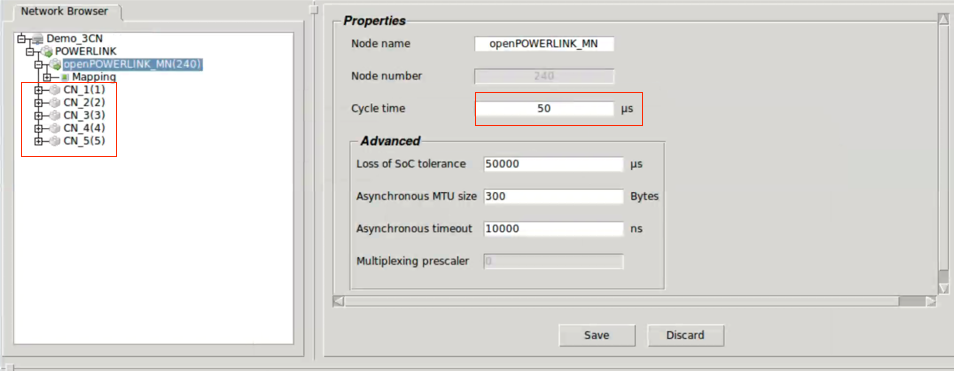
\includegraphics[width=\textwidth]{openconfigurator.png}
  \caption{openconfigurator主界面}
  \label{fig:openconfigurator}
\end{figure}

图~\ref{fig:cn1-setting}为openCONFIGURATOR中1号从站的配置界面,值得注意的是从站的PollResponse Timeout网络参数,这个是指主站接收该从站PRes数据桢的超时时间。网络中的从站有可能发生故障,导致从站无法发送数据或者发送的数据无法到达主站,如果主站在PollResponse Timeout这个时间段内没有收到该从站的回复数据时,就会将该节点略过,和下一个节点通信。此外,如果从站设备的反应时间很长,那么就需要将PollResponse Timeout参数设置的大一些,例如如果该从站基于FPGA,这个参数设置为2\~{}20$\mu$s均可,如果该从站基于windows,这个参数可能要设置为几个ms。

\begin{figure}[!htb]
  \centering
  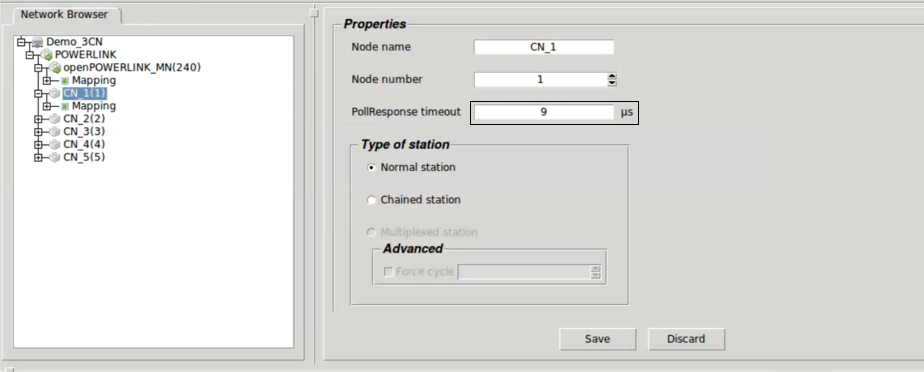
\includegraphics[width=\textwidth]{cn1-setting.png}
  \caption{1号从站的配置界面}
  \label{fig:cn1-setting}
\end{figure}

\subsection{基于Linux系统实现POWERLINK协议}

openPOWERLINK不需要额外硬件就可以直接运行在基于x86架构的Linux系统平台下,为了减小Linux系统对openPOWERLINK实时性能的影响,我们为linux系统安装了RT-PREEMPT实时补丁。根据协议栈运行位置的不同,openPOWERLINK在实时Linux系统下有两种工作模式\cite{wallner}:\\
(1) 协议栈工作在用户空间:协议栈被封装成一个运行于用户空间的用户代码库,通过调用libcap library来访问以太网接口。这种工作模式的优点是支持所有标准以太网的网卡芯片。这种工作模式的实时性能在1ms左右,可以满足大多数应用场景。\\
(2) 协议栈工作在内核空间:协议栈直接工作在Linux内核空间下,直接访问以太网硬件接口,实时性高。这种工作模式的缺点是对以太网硬件接口依赖严重,需要针对不同的网口类型开发相应的驱动程序,限制了openPOWERLINK的应用。\\


本小节对工作在用户空间的POWERLINK协议栈进行了性能测试,内核模式下的高性能方案在第~\ref{section:主站PC方案的系统设计与开发}节中详细介绍。

我们建立由2台RT-Linux PC构成的简单系统,系统架构如图~\ref{fig:linux-powerlink-test}所示,一台用作POWERLINK主站,一台是节点号为1的从站,主站和从站均运行V2.2.2版本的openPOWERLINK开源程序,节点之间采用千兆POWERLINK通信。

\begin{figure}[!htb]
  \centering
  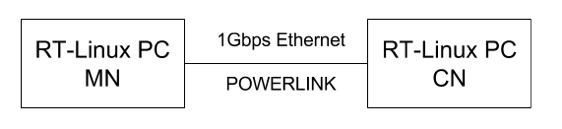
\includegraphics[width=0.8\textwidth]{linux-powerlink-test.png}
  \caption{基于RT-Linux PC的POWERLINK通信测试系统}
  \label{fig:linux-powerlink-test}
\end{figure}

openPOWERLINK程序的安装与启动过程如下所示:

\begin{lstlisting}
1.安装cmake编译工具
下载cmake-3.5.0-rc3.tar.gz并解压
> cd <cmake_dir>
> ./bootstrap
> make
> make install

2.编译openPOWERLINK协议栈
下载openPOWERLINK_V2.2.2.tar.gz并解压
Create debug libraries
> cd <openPOWERLINK_dir>/stack/build/linux
> cmake -DCMAKE_BUILD_TYPE=Debug ../..
> make
> make install
Create release libraries
> cd <openPOWERLINK_dir>/stack/build/linux
> cmake -DCMAKE_BUILD_TYPE=Release ../..
> make
> make install


3.编译openPOWERLINK应用层程序
> cd <openPOWERLINK_dir>/apps/<demo_dir>/build/linux
> cmake ../..
> make
> make install


4.将配置文件mnobd.cdc拷贝至主站的启动目录下
[test@powerlinkTest1 demo_mn_console]$ ls
demo_mn_console  mnobd.cdc  mnobd.cdc-bk  set_prio

5.启动openPOWERLINK
主站启动:
[test@powerlinkTest1 demo_mn_console]$ sudo ./demo_mn_console
从站启动:
[test@powerlinkTest2 demo_cn_console]$ sudo ./demo_mcn_console

\end{lstlisting}

我们将测试系统通信周期配置为1ms,系统可以稳定运行,图~\ref{fig:wireshark-pc-test}是抓取的POWERLINK协议帧数据。如图~\ref{fig:wireshark-pc-test}所示,在1ms的通信周期内,主站和从站严格按照PReq/PRes的轮询响应模式进行通信,通过两个连续SoC帧之间的间隔可以计算得到通信周期。我们抓取了25万个连续的POWERLINK数据帧,并绘制了如图~\ref{fig:pc-soc-cycle-density}所示的概率密度分布图,该图表明,大多数的通信周期接近1ms,实时性一般,抖动较大。

\begin{figure}[!htb]
  \centering
  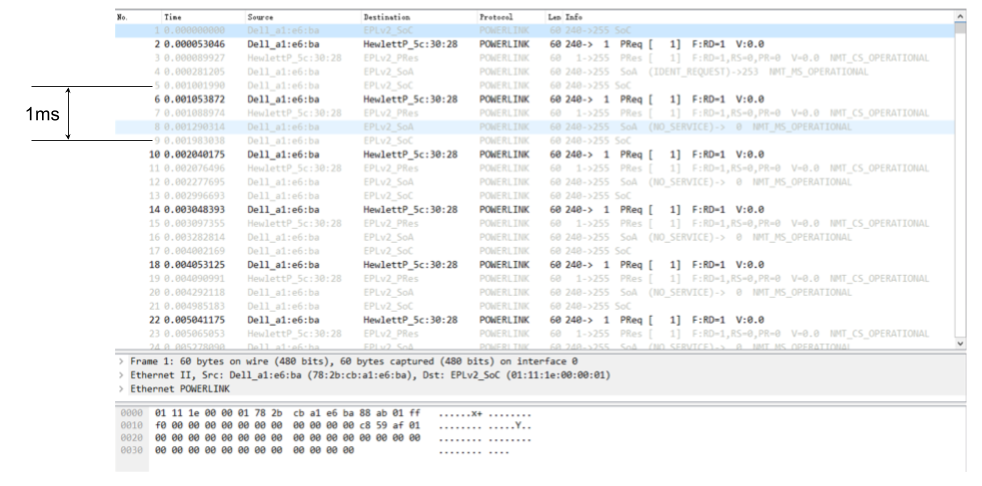
\includegraphics[width=\textwidth]{wireshark-pc-test.png}
  \caption{基于两台PC的wireshark抓包结果}
  \label{fig:wireshark-pc-test}
\end{figure}

\begin{figure}[!htb]
  \centering
  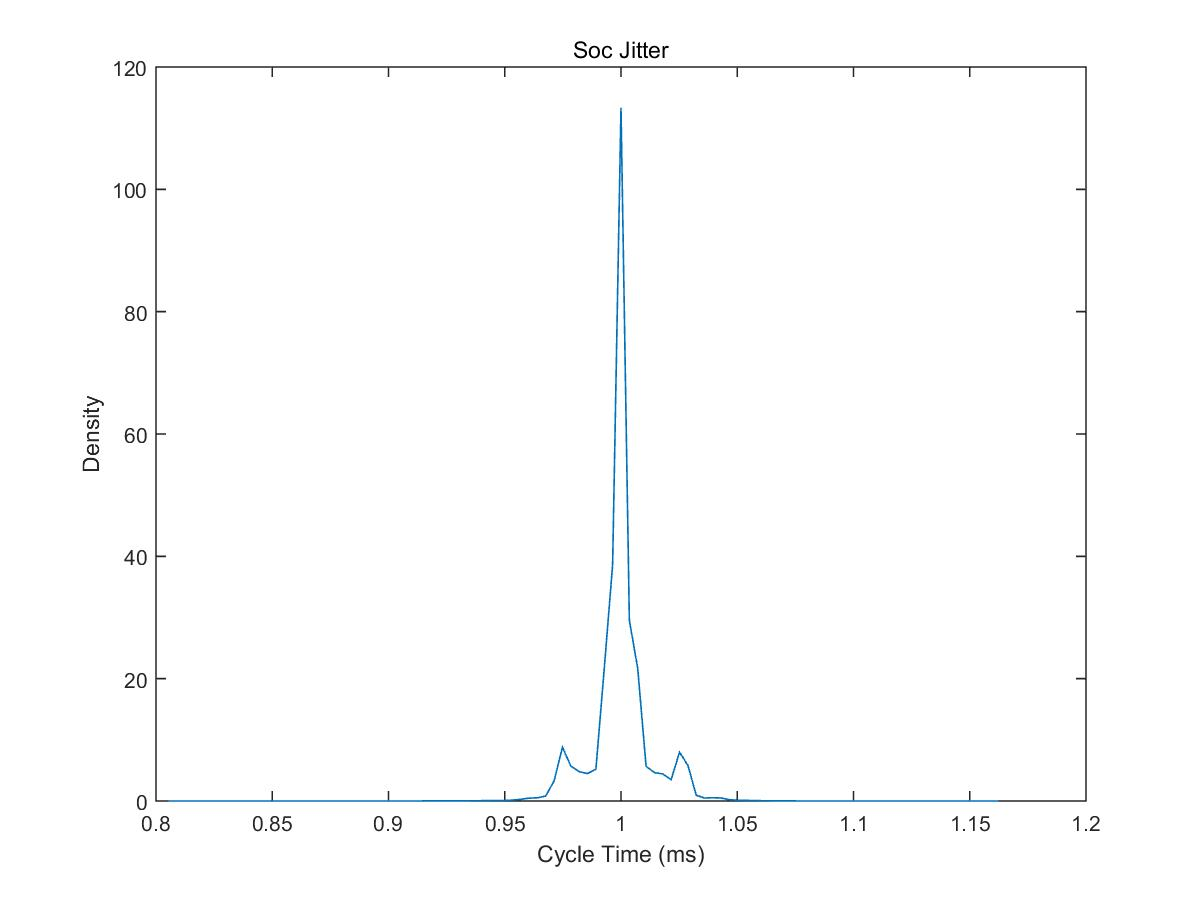
\includegraphics[width=\textwidth]{pc-soc-cycle-density.png}
  \caption{基于两台PC的通信周期概率密度分布图}
  \label{fig:pc-soc-cycle-density}
\end{figure}

\subsection{基于FPGA实现POWERLINK协议}
\label{subsection:基于FPGA实现POWERLINK协议}

基于FPGA实现POWERLINK协议的方案有两种\cite{xiao}:\\
(1) 软核方案:在FPGA中的MCU上运行POWERLINK协议栈,MCU为软核(例如:Altera Nios,Xilinux Zynq),软核中运行的是openPOWERLINK的协议栈,循环周期可以达到100\~{}200$\mu$s。\\
(2) HDL方案:采用纯硬件描述语言HDL来实现POWERLINK的协议栈,这种方案不需要MCU,实时性能较高,循环周期可以达到数十$\mu$s。

本小节主要介绍软核方案的技术细节和测试结果,HDL方案在第~\ref{section:全站FPGA方案的系统设计与开发}中详细介绍。软核方案实现的硬件平台是友晶科技的DE2-115的FPGA开发板,DE2-115开发板具有充足的逻辑处理单元和存储单元,同时兼具低功耗、低成本的优点,具体配置如下:\\
(1) 核心的FPGA芯片:FPGACyclone IV 4CE115F29,包含有115k个逻辑单元,低成本,低功耗。\\
(2) 存储单元: 2-Mbyte SRAM,64-Mbyte SDRAM,8-Mbyte Flash memory。
(3) 时钟:50M晶振,支持外部时钟。
(4) 标准接口:2个100M自适应以太网络适配器,80针带保护电路的外接IO,通用串行总线USB接口,SD Card接口,RS-232标准串口。

软件基于Altera Nios II软核来实现,Nios II是由Altera公司推出的嵌入式软核处理器,它采用32位精简指令集,32位数据通道,可在一个时钟周期内完成一条指令的处理。作为目前最流行的软核处理器Nios II核拥有高计算性能,但占用不到50\%的FPGA资源。同时Altera公司提供了与Nios II配套的软件集成开发环境Quartus II,可以在该环境下完成包括编辑、编译、调试程序和下载在内的软件开发任务。

基于Nios II软核的POWERLINK协议软件架构如图~\ref{fig:oplk-de2-115-arch}所示。软核处理器Altera Nios II被实例化为POWERLINK通信处理器(Communication Processor)和主机处理器(host processor),这两个软核分别用来执行openPOWERLINK内核层和用户层的代码。处理器之间通过Altera Avalon总线连接。以太网接口是通过优化控制器openMAC构建的,此外,还实现了一个集线器(HUB)软核,用来组建菊花链拓扑结构的网络。

采用软核方案来实现POWERLINK,通信过程如下:\\
第一步:主站的PReq数据桢通过以太网的openMAC发送到从站。\\
第二步:从站的以太网openMAC收到数据桢以后,向POWERLINK通信处理器和主机处理器发起中断,请求处理器处理收到的数据桢。\\
第三步:处理器响应中断请求,处理PReq数据桢,并回复PRes数据桢。在这个过程中,处理器响应中断请求并处理中断的时间比较长,往往在几十个$\mu$s。

\begin{figure}[!htb]
  \centering
  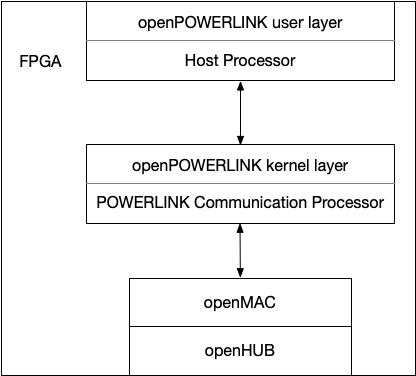
\includegraphics[width=0.7\textwidth]{oplk-de2-115-arch.png}
  \caption{基于DE2-115开发板的POWERLINK软件架构图}
  \label{fig:oplk-de2-115-arch}
\end{figure}

基于软核方案,我们设计了由1个主站和6个从站组成的系统,系统架构如图~\ref{fig:de2-115-test-arch}所示。该系统是线性拓扑结构,从站按照节点号从小到大的顺序依次连接。主站是RT-Linux PC,从站是DE2-115开发板,节点之间基于百兆POWERLINK通信\cite{xksun-2018}。

\begin{figure}[!htb]
  \centering
  
\includegraphics[width=0.85\textwidth]{de2-115-test-arch.png}
  \caption{基于DE2-115开发板的POWERLINK通信测试系统}
  \label{fig:de2-115-test-arch}
\end{figure}

对于POWERLINK测试系统,我们采用Hilscher netAnalyzer以太网分析仪用来抓取POWERLINK数据帧。以太网分析仪netANALYZER是用于对实时以太网传输数据进行监控和分析的工具,由德国赫优讯公司生产。Hilscher netANALYZER由于其内置的ASIC专用芯片,测量分辨率可达到10ns,可以用来测量各种高精度时间同步协议,如:IEEE1588、PROFINET IRT、EtherNet/IP 集成CIP Sync、EtherCAT或 Sercos、Ethernet POWERLINK。Hilscher netANALYZER在硬件上集成的测试访问点Tap,保证了测试过程中以太网通信不会受到影响,既不会带来额外的数据帧延时,也不影响时间抖动。测试访问点Tap还保证了即使在错误状态下数据内容也不会被改变。网络上发生的所有报文数据及报文错误都毫无改变地传输至现场设备。如图~\ref{fig:netANALYZER-photo}所示的以太网分析仪netANALYZER包含5个以太网端口,其中2个“Tap”端口组成“TapA”,2个“Tap”端口组成“TapB”,可以同时抓取2条通信网络上的数据帧。另一个端口作为“镜像端口”负责接收来自TapA/TapB端口上的转发数据,同时“镜像端口”负责将数据传输至与PC,PC上运行了专用软件netANALYZER Scope2,支持将抓包结果输出为可被Wireshark解析的pcap格式文件,从而可以进行更详细的分析。这里我们仅用到了“TapA”端口进行POWERLINK通信测试。

\begin{figure}[htb]\centering
  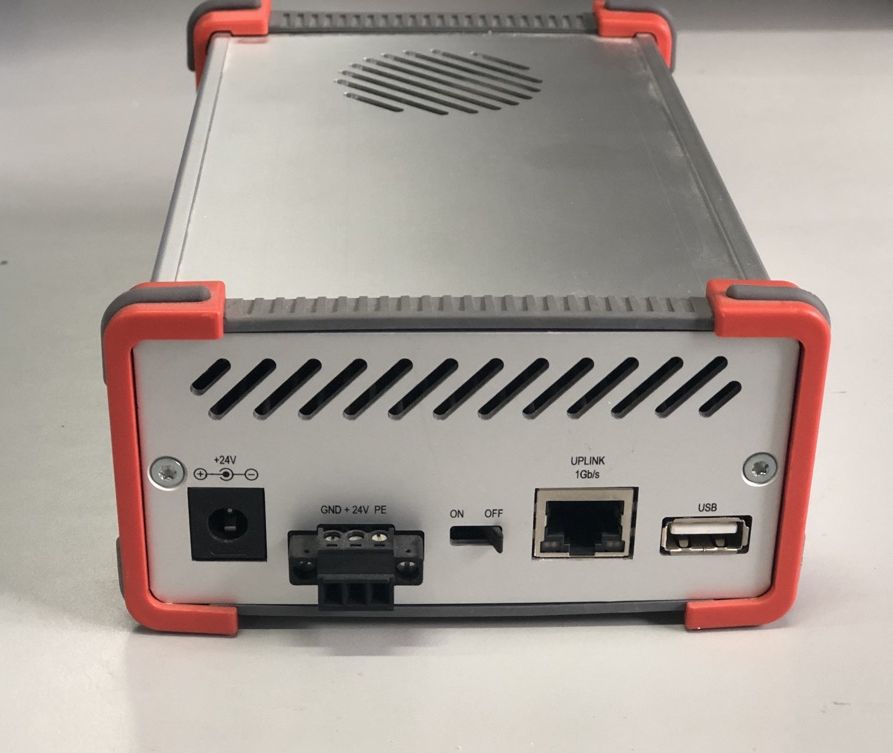
\includegraphics[width=.452\textwidth]{netANALYZER_1.png}  
  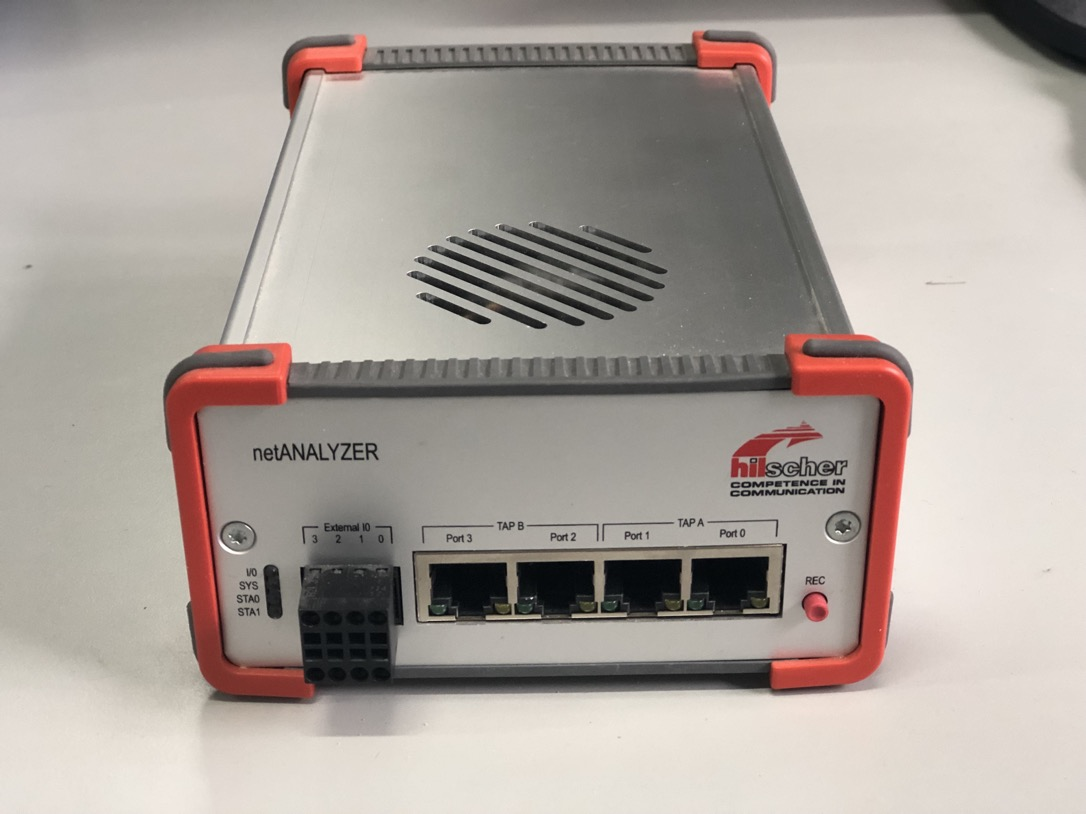
\includegraphics[width=.508\textwidth]{netANALYZER_2.jpg}
  \caption{以太网分析仪netANALYZER正面(左图)和背面(右图)}
  \label{fig:netANALYZER-photo}
\end{figure}


基于此设计,我们搭建了如图~\ref{fig:de2-115-photo}所示的测试系统。其中,PC的操作系统是带有实时补丁rtai-3.10.75的Centos7.4.1708,PC上的openPOWERLINK程序工作在用户空间。示波器用来测试系统响应时间,我们采用Hilscher netAnalyzer以太网分析仪用来抓取POWERLINK数据帧,这里我们仅用到了“TapA”端口进行POWERLINK通信测试。
\begin{figure}[!htb]
  \centering
  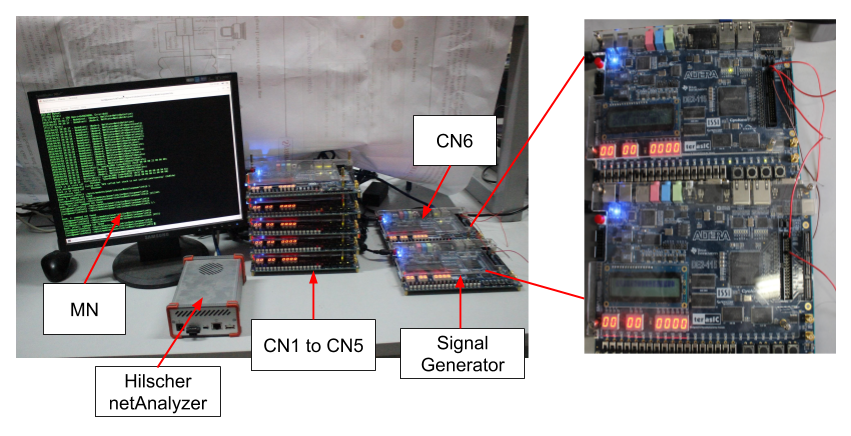
\includegraphics[width=\textwidth]{de2-115-photo.png}
  \caption{基于DE2-115开发板的POWERLINK通信系统实物图}
  \label{fig:de2-115-photo}
\end{figure}

基于此测试系统,我们进行了通信周期和响应时间的性能测试。经过多次测试,该系统可以在700$\mu$s的通信周期下的稳定运行,Hilscher netAnalyzer以太网分析仪的抓包结果如图~\ref{fig:de2-115-wireshark}所示。我们测试了大约27000个连续的POWERLINK通信周期,循环周期的平均值约为703$\mu$s,图~\ref{fig:de2-115-density}是python程序拟合的通信周期的概率密度分布曲线,密度的峰值在通信周期为700$\mu$s附近,但是抖动较大。

\begin{figure}[!htb]
  \centering
  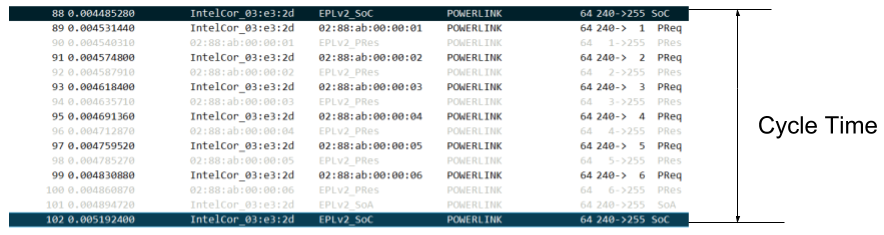
\includegraphics[width=\textwidth]{de2-115-wireshark.png}
  \caption{基于DE2-115开发板的的wireshark抓包结果}
  \label{fig:de2-115-wireshark}
\end{figure}

\begin{figure}[!htb]
  \centering
  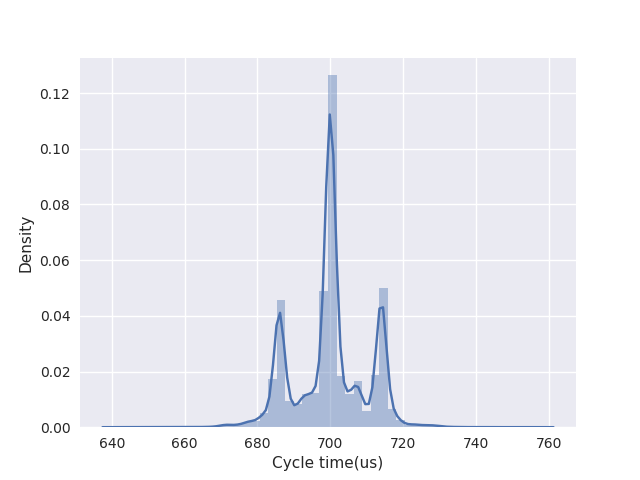
\includegraphics[width=\textwidth]{de2-115-density.png}
  \caption{基于DE2-115开发板的通信周期概率密度分布图}
  \label{fig:de2-115-density}
\end{figure}

响应时间是输入信号到达系统和系统回复输出信号之间的时间差。 它包括DE2-115开发板上输入/输出信号的处理时间,数据通信时间,网线延迟和集线器延迟。 数据通信时间是主要部分,其他时间在1\~{}10$\mu$s的水平。对于此测试系统,在一个通信周期中,从站1是第一个开始通信的从站,从站6是最后一个结束通信的从站,所以从站1输入信号到从站6输出信号的时间差是最长的通信时间,即是系统最长响应时间。完成的响应过程如下:\\
第一步:在第n个周期中,从站1的输入信号通过PRes数据帧进行POWERLINK网络。\\
第二步:主站收到从站1的PRes数据帧后,对输入信号进行相应的处理。\\
第三步:在第n+1个周期中,主站通过PReq数据帧将输出数据传输给从站6,从站6输出相应信号。

我们使用示波器测试了该测试系统的最长响应时间,图~\ref{fig:de2-115-response-time}是示波器在“单触发”模式下的测试结果,通道2(ch2)是从站1的输入信号,通道1(ch1)是从站6的输出信号。响应时间约为1070$\mu$s,

\begin{figure}[!htb]
  \centering
  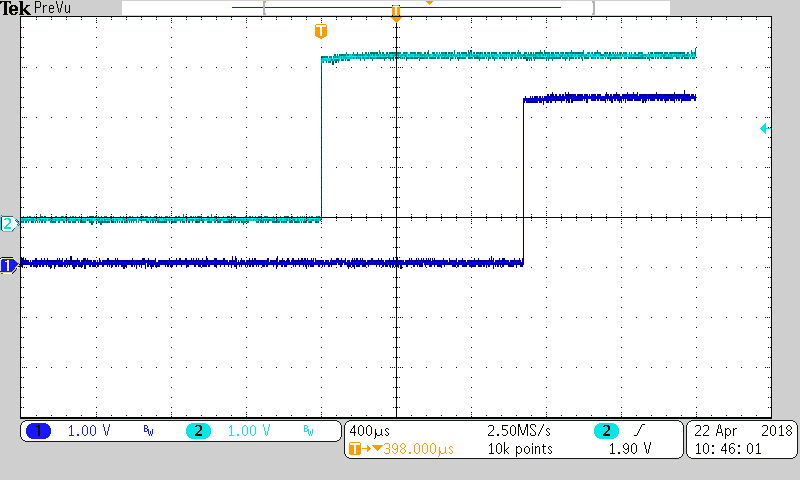
\includegraphics[width=\textwidth]{de2-115-response-time.png}
  \caption{基于DE2-115开发板的测试系统响应时间测试结果}
  \label{fig:de2-115-response-time}
\end{figure}

\subsection{测试小结}

本节分析了openPOWERLINK的两种实现方式,分别是Linux用户空间方案和基于FPGA的软核方案。针对两种实现方式我们分别搭建了测试系统并进行相关性能测试,根据测试结果,总结如下:\\
(1) 在Linux用户空间方案中,通信周期最快为1ms;在基于FPGA的软核方案中,七个节点的系统通信周期最快为700$\mu$s。POWERLINK协议在FPGA硬件平台下的实时性能明显优于在x86 Linux平台下的性能。\\
(2) 对于基于FPGA的软核方案,如图~\ref{fig:de2-115-wireshark}所示,相邻PRes数据帧和PReq数据帧为FPGA从站响应时间,反应时间约为10$\mu$s左右,这是由于软核处理PReq数据桢并回复PRes数据桢而导致的延时。若采用纯硬件描述语言HDL来实现POWERLINK的协议栈可缩短从站的响应时间,进而提高实时性能。\\
(3) 在数据传输速度上,百兆以太网比千兆以太网低一个量级,所以POWERLINK物理层采用千兆以太网可以减少数据传输的延时。\\
(4) 通过以下三种方式可以进一步提高实时性:\\
        • openPOWERLINK工作在Linux系统的内核空间下。\\
        • 在FPGA平台下,采用纯硬件描述语言HDL来实现POWERLINK的协议栈。\\
        • POWERLINK物理层采用千兆以太网。

\section{POWERLINK通信周期的理论计算}
\label{section:理论计算POWERLINK通信周期}
通信周期直接反应系统的实时性,决定了系统的响应时间。我们提出了理论分析和仿真模拟两种方法,同时结合系统的实际通信参数,来预估多节点POWERLINK系统的通信周期,从而为多节点大规模的POWERLINK方案设计提供依据。本节首先详细分析POWERLINK通信周期的时间组成,最后推导出通信周期的计算公式\cite{Knezic2017}。

\begin{figure}[!htb]
  \centering
  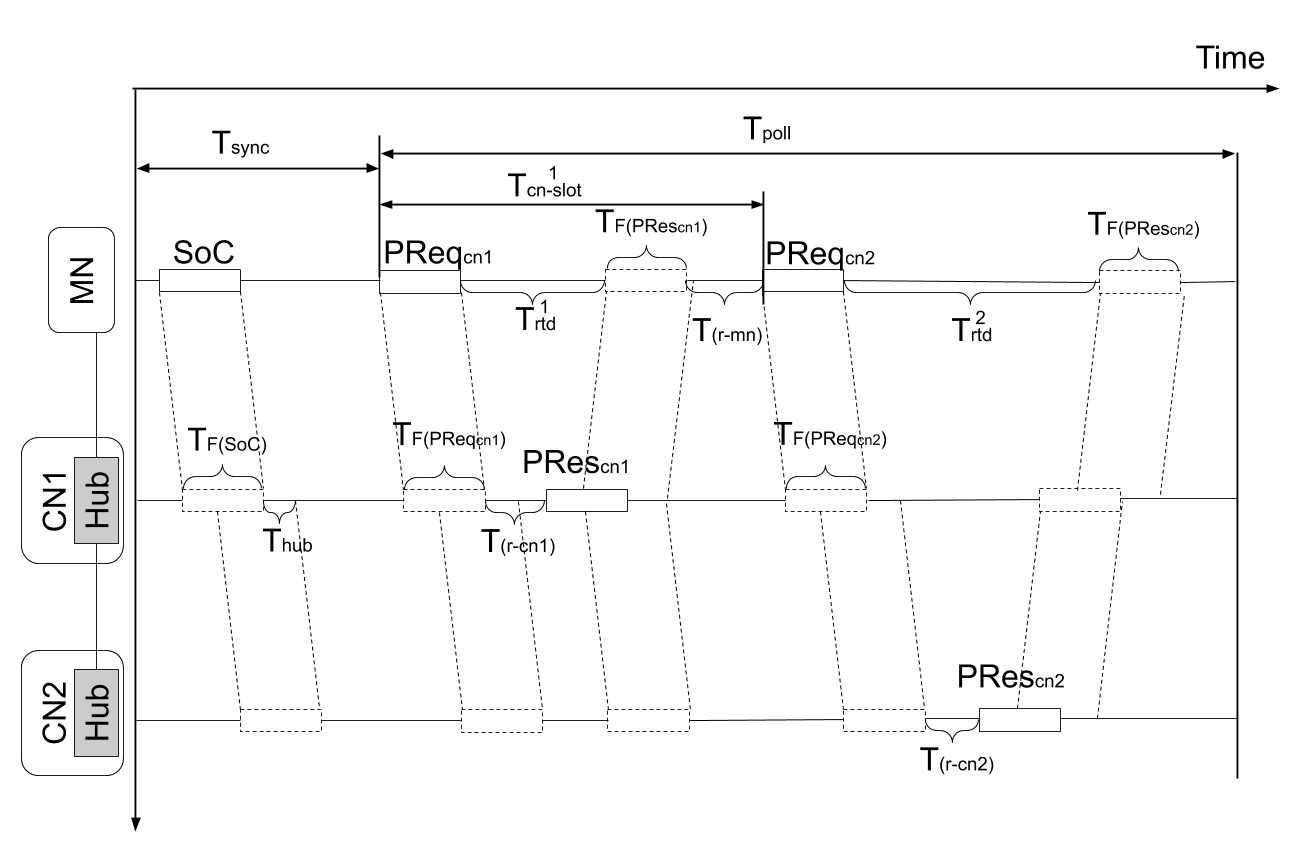
\includegraphics[width=\textwidth]{powerlink-communication-process.png}
  \caption{powerlink等时同步阶段通信过程}
  \label{fig:powerlink-communication-process}
\end{figure}

在POWERLINK通信周期中,等时同步阶段用来传输周期性的实时数据,占据了绝大部分的通信周期。图~\ref{fig:powerlink-communication-process}表示了一个基本POWERLINK网络的等时同步通信过程,该POWERLINK网络由一个主站和两个从站组成,各站点按照线型拓扑连接。等时同步阶段由同步阶段和轮询阶段组成,如公式~\ref{equation1}所示,其中$T_{ip}$代表等时同步阶段时间,$T_{sync}$和$T_{poll}$分别代表同步阶段和轮询阶段的时间。$T_{sync}$由公式~\ref{equation2}表示,$T_{F(SoC)}$为同步数据帧传输的时间。根据第~\ref{subsection:POWERLINK协议的网络模型}中对POWERLINK数据帧的分析,SoC帧的大小为64Byte,采用千兆以太网传输,$T_{F(SoC)}$仅为0.512$\mu$s,$T_{W}$为等待从站接收并处理SoC帧的时间,一般来说$T_{W}$的大小取决于从站的配置。

\begin{equation}
\label{equation1}
T_{ip}=T_{sync}+T_{poll}
\end{equation}

\begin{equation}
\label{equation2}
T_{sync}=T_{F(SoC)}+T_{W}
\end{equation}

轮询阶段时长($T_{poll}$)可由公式~\ref{equation3}表示,$T_{frames}$为轮询阶段中所有数据帧的传输时间,$T_{net}$为由所有网络组件造成的延时,网络组件包括主站、从站、HUB和网线。如图~\ref{fig:powerlink-communication-process}所示,PReq和PRes数据帧在每个从站时隙都会被发送,$T_{frames}$可以用公式~\ref{equation4}表示。

\begin{equation}
\label{equation3}
T_{poll}=T_{frames}+T_{net}
\end{equation}

\begin{equation}
\label{equation4}
T_{frames}=\sum_{i=1}^n(T_{F(PReq)}^{i}+T_{F(PRes)}^{i})
\end{equation}

\begin{equation}
\label{equation5}
T_{net}=\sum_{i=1}^nT_{rtd}^{i}+nT_{r-mn}
\end{equation}

$T_{net}$由公式~\ref{equation5}表示,如图~\ref{fig:powerlink-communication-process}所示,$T_{rtd}^{i}$为主站在第i个从站时间间隙内的往返延时,$T_{r-mn}$为主站的响应时间。对于图~\ref{fig:powerlink-communication-process}所示的POWERLINK网络结构,$T_{rtd}^{1}$和$T_{rtd}^{2}$分别由公式~\ref{equation6}和~\ref{equation7}表示,其中$T_{c}$为网线传播延时,$T_{hub}$为从站控制器的HUB延时,$T_{r-cni}$为第i个从站的处理时间。根据公式~\ref{equation6}和~\ref{equation7},$T_{rtd}^{i}$可用公式~\ref{equation8}所示,当从站设备类型相同,$T_{r-cni}$都等于$T_{r-cn}$。

\begin{equation}
\label{equation6}
T_{rtd}^{1}=2T_{c}+T_{hub}+T_{r-cn1}
\end{equation}

\begin{equation}
\label{equation7}
T_{rtd}^{2}=4T_{c}+3T_{hub}+T_{r-cn2}
\end{equation}

\begin{equation}
\label{equation8}
T_{rtd}^{i}=2iT_{c}+(2i-1)T_{hub}+T_{r-cn}
\end{equation}

\begin{equation}
\label{equation9}
\sum_{i=1}^ni=n(n+1)/2
\end{equation}

我们假设所有的从站设备类型相同且使用等长网线连接,即对于每个从站来说,参数$T_{c}$,$T_{hub}$和$T_{r-cn}$均相等。将公式~\ref{equation8}和公式~\ref{equation9}代入公式~\ref{equation5},可得公式~\ref{equation10},$T_{net}^{line}$为线性拓扑结构下所有网络组件造成的延时。

\begin{equation}
\begin{split}
\label{equation10}
T_{net}^{line}&=\sum_{i=1}^n[2iT_{c}+(2i-1)T_{hub}+T_{r-cn}]+nT_{r-mn}\\
&=n(n+1)T_{c}+n^2T_{hub}+n(T_{r-cn}+T_{r-mn})
\end{split}
\end{equation}

将公式~\ref{equation4}的值和公式~\ref{equation10}代入公式~\ref{equation3},可得到轮询阶段时长($T_{poll}$)的值,如公式~\ref{equation11}所示:

\begin{equation}
\begin{split}
\label{equation11}
T_{poll}=\sum_{i=1}^n(T_{F(PReq)}^{i}+T_{F(PRes)}^{i}) + n(n+1)T_{c}+n^2T_{hub}+n(T_{r-cn}+T_{r-mn})
\end{split}
\end{equation}

考虑到同步阶段时长和空闲阶时长$T_{idle}$,可得循环周期$T_{cycle\_time}$,如公式~\ref{equation12}所示:

\begin{equation}
\label{equation12}
T_{cycle\_time}=T_{F(SoC)}+T_{W}+\sum_{i=1}^n(T_{F(PReq)}^{i}+T_{F(PRes)}^{i}) + n(n+1)T_{c}+n^2T_{hub}+ n(T_{r-cn}+T_{r-mn})+T_{idle}
\end{equation}

这里$T_{c}$,$T_{hub}$、$T_{r-cn}$和$T_{r-mn}$等参数与网线长度、主站从站的配置有关,需要根据具体情况来确定。

同时需要另外注意的一个参数是各从站的通信时隙$T_{cn-slot}^{i}$,我们可以根据$T_{cn-slot}^{i}$的值来配置openCONFIGURATOR来配置PollResponse Timeout参数,PollResponse Timeout参数的值要大于$T_{cn-slot}^{i}$的值。如图~\ref{fig:powerlink-communication-process}所示,$T_{poll}$为各从站的通信时隙$T_{cn-slot}^{i}$之和,$T_{poll}$也可以用公式~\ref{equation13}表示。根据图~\ref{fig:powerlink-communication-process}所示,$T_{cn-slot}^{i}$可用公式~\ref{equation14}表示。

\begin{equation}
\label{equation13}
T_{poll}^{i}=\sum_{i=1}^nT_{cn-slot}^{i}
\end{equation}

\begin{equation}
\label{equation14}
T_{cn-slot}^{i}=T_{F(PReq)}^{i}+T_{F(PRes)}^{i}+T_{rtd}^{i}+T_{r-mn}
\end{equation}

\section{POWERLINK通信协议的仿真模拟}
\label{section:仿真模拟POWERLINK通信协议}

\subsection{OMNeT++仿真器}
通过对POWERLINK系统的通信过程理论分析,我们得到通信周期的计算公式,可以对POWERLINK系统的实时性能进行初步估算。为了进一步准确可靠的评估POWERLINK通信系统性能,我们还发展了仿真建模的分析方法。POWERLINK网络仿真基于OMNet++网络模拟器展开,OMNeT++(Objective Modular Network Testbed in C++)是一个面向对象的模块化离散事件网络仿真框架\cite{omnet}。作为面向对象的离散事件仿真器,OMNeT++主要用于通信网络和分布式系统的仿真,具体可以应用于以下领域\cite{gao2015,xu2014,liu2015}:\\
(1) 协议建模;\\
(2) 有线和无线通信网络的建模;\\
(3) 排队网络建模;\\
(4) 多处理器等分布式硬件系统的建模;\\
(5) 验证硬件架构;\\
(6) 评估复杂软件系统的性能。

OMNeT++模型的基本元素是基于C++实现的简单模块,简单模块中可以定义消息格式和消息传播的行为,简单模块之间通过门和连接相互通信,从而形成复杂模块,复杂模块可以由无限个简单模块构成,多个复杂模块组成整个OMNeT++模型。在下面的图~\ref{fig:omnet-model}中,方框代表简单的模块(灰色背景)和复合模块,小方块表示门,箭头表示连接\cite{wu2006}。
\begin{figure}[!htb]
  \centering
  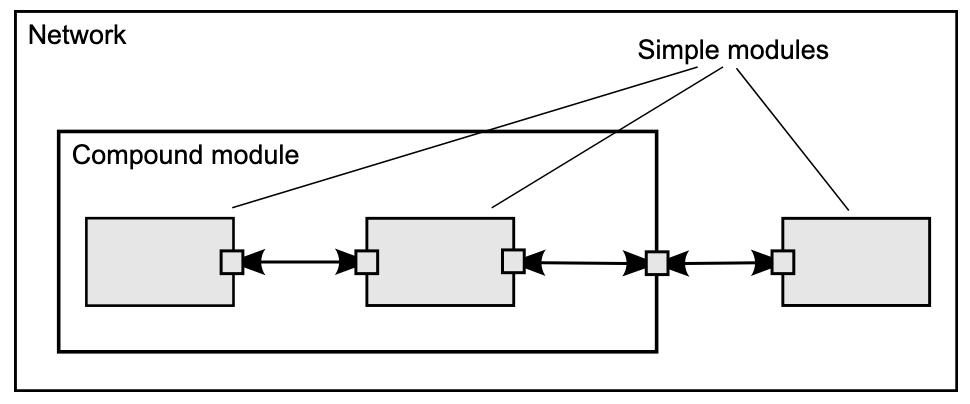
\includegraphics[width=\textwidth]{omnet-model.png}
  \caption{omnet简单模块与复杂模块}
  \label{fig:omnet-model}
\end{figure}

OMNeT++的主要组成部分如下:\\
(1) 仿真内核库:OMNeT++提供的仿真类库代码;\\
(2) 网络拓扑描述文件:由NED语言编写的文件,既可以用来描述网络拓扑结构,又可以通过参数、门、信道连接、简单模块等来定义复杂模块;\\
(3) 消息定义文件:用于定义数据报文格式;\\
(4) 简单模块定义文件:简单模块的行为定义文件,包括C++编写的*.cc文件和*.h\\
(5) 用户接口:该接口用于仿真运行时的测试,演示等工作。

在使用OMNeT++建模中,最常使用的就是INET框架。INET框架是开源的OMNeT++的标准协议模型库,对应OMNeT的各种新版本INET框架还在不断更新中,INET框架包含了常用的多种有线和无线协议的模型,具体到各种物理层模型、应用层模型等。在POWERLINK仿真建模中,我们使用的是OMNeT++4.6版本搭配inet-2.6-b673687版本。

\subsection{POWERLINK通信节点建模}

\begin{figure}[!htb]
  \centering
  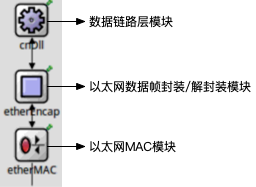
\includegraphics[width=0.6\textwidth]{powerlink-model.png}
  \caption{POWERLINK通信节点模型}
  \label{fig:powerlink-model}
\end{figure}
基于OMNeT++仿真平台,我们对POWERLINK主站和从站进行了建模。节点模型如图~\ref{fig:powerlink-model}所示,由以下三个模块组成:\\
(1) 以太网MAC模块:采用INET框架下的标准以太网MAC模块,支持千兆以太网通信;\\
(2) 以太网数据帧封装/解封装模块:采用INET框架下的EtherEncap模块,用于EthernetII数据帧的封装和解封装;\\
(3) 数据链路层模块:按照POWERLINK的SCNM机制定义了模块行为。

我们在配置文件中定义了各节点模型的通信参数,主要的配置文件包括omnetpp.ini和xdc\_cn\_std.xml文件,其中omnetpp.ini文件中定义了POWERLINK模型的通信周期、主站从站的响应时间以及从站的节点号和响应数据大小,具体如下所示:

\begin{lstlisting}
# The configuration of the MN
POWERLINK模型的通信周期:
**.MN.mnDll.cycleLenMean = 500us
主站响应时间:
**.MN.mnDll.responseTimeMean = 1us

# The configuration of the CNs
从站响应时间:
**.CN.cnDll.responseTimeMean = 1us
1号从站的节点号以及响应数据大小:
**.CN1.cnDll.nodeId = 1
**.CN1.cnDll.presActPayload = 1

2号从站的节点号以及响应数据大小:
**.CN2.cnDll.nodeId = 2
**.CN2.cnDll.presActPayload = 1

# The configuration of the hub
hub延时:
**.hubDelayMean = 50ns
\end{lstlisting}


xdc\_cn\_std.xml文件中则定义了各从站的通信间隙(PResTimeout)以及接收来自主站请求数据帧的大小(PReqActPayload),这里“PResTimeout”参数的意义与openCONFiGURATOR中设置的PollResponse Timeout网络参数意义相同。
\begin{lstlisting}
<Nodes>
  <Node NodeId="1" PResTimeout="6000ns" PReqActPayload="1" />
  <Node NodeId="2" PResTimeout="9000ns" PReqActPayload="1" />
</Nodes>
\end{lstlisting}



除了对通信节点建模之外,在.msg文件中定义四种POWERLINK数据帧结构。
\begin{lstlisting}
cplusplus {{
// POWERLINK node reserved addresses
const int C_ADR_INVALID = 0;
const int C_ADR_MN_DEF_NODE_ID = 240;
const int C_ADR_DUMMY_NODE_ID = 252;
const int C_ADR_DIAG_DEF_NODE_ID = 253;
const int C_ADR_RT1_DEF_NODE_ID = 254;
const int C_ADR_BROADCAST = 255;
// POWERLINk messages header size (in bytes)
const int EPL_SOC_HEADER_BYTES = 46;
const int EPL_PREQ_HEADER_BYTES = 10;
const int EPL_PRES_HEADER_BYTES = 10;
const int EPL_SOA_HEADER_BYTES = 46;
const int EPL_ASND_HEADER_BYTES = 4;
}}

enum eMsgType
{
    MsgTypeNonPowerlink = 0x00;
    MsgTypeSoc = 0x01;
    MsgTypePreq = 0x03;
    MsgTypePres = 0x04;
    MsgTypeSoa = 0x05;
}

packet POWERLINkHdr {
    int MsgType enum(eMsgType);
    int Dst;
    int Src;
}

packet SocFrame extends POWERLINkHdr {
    MsgType = MsgTypeSoc;
    Dst = C_ADR_BROADCAST;
    Src = C_ADR_MN_DEF_NODE_ID;
    bool MC;
    bool PS;
    long NetTime;
    long RelativeTime;
}

packet SoaFrame extends POWERLINkHdr {
    MsgType = MsgTypeSoa;
    Dst = C_ADR_BROADCAST;
    Src = C_ADR_MN_DEF_NODE_ID;
    int NMTStatus;
    int RequestedServiceID;
    int RequestedServiceTarget;
    int EPLVersion;
}

packet PreqFrame extends POWERLINkHdr {
    MsgType = MsgTypePreq;
    Src = C_ADR_MN_DEF_NODE_ID;
    bool MS;
    bool EA;
    bool RD;
    int PDOVersion;
    int Size;
}

packet PresFrame extends POWERLINkHdr {
    MsgType = MsgTypePres;
    Dst = C_ADR_BROADCAST;
    int NMTStatus;
    bool MS;
    bool EN;
    bool RD;
    int PR;
    int RS;
    int PDOVersion;
    int Size;
}
\end{lstlisting}

我们只需要通过编写.ned文件来定义相应系统拓扑结构,代入主从节点模型以及相应参数即可对相应的POWERLINK通信系统进行模拟。
